\chapter{Parte teórica y desarrollo del código}
El paquete \texttt{solaR2} toma como marco teórico el libro de Oscar Perpiñán, tutor de este trabajo, Energía Solar Fotovoltaica \cite{Perpinan2023} para cada una de las operaciones de cálculo que realizan cada una de las funciones.
En la figura \ref{fig:orgd529198}, se muestra un diagrama que resume los pasos que se siguen a la hora de calcular la producción de sistemas fotovoltaicos.
\begin{figure}[t]
\centering
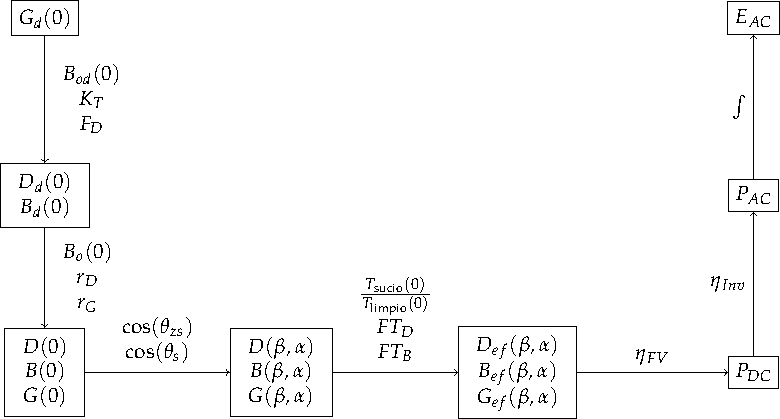
\includegraphics[scale=0.6]{figuras/ProcedimientoCalculoRadiacionInclinada.pdf}
\caption{\label{fig:orgd529198}Procedimiento de cálculo}
\end{figure}

En la figura \ref{fig:orgc6e945c}, se muestra el proceso de cálculo que sigue el paquete a la hora de obtener la estimación de la producción del sistema fotovoltaico
\begin{figure}[t]
\centering
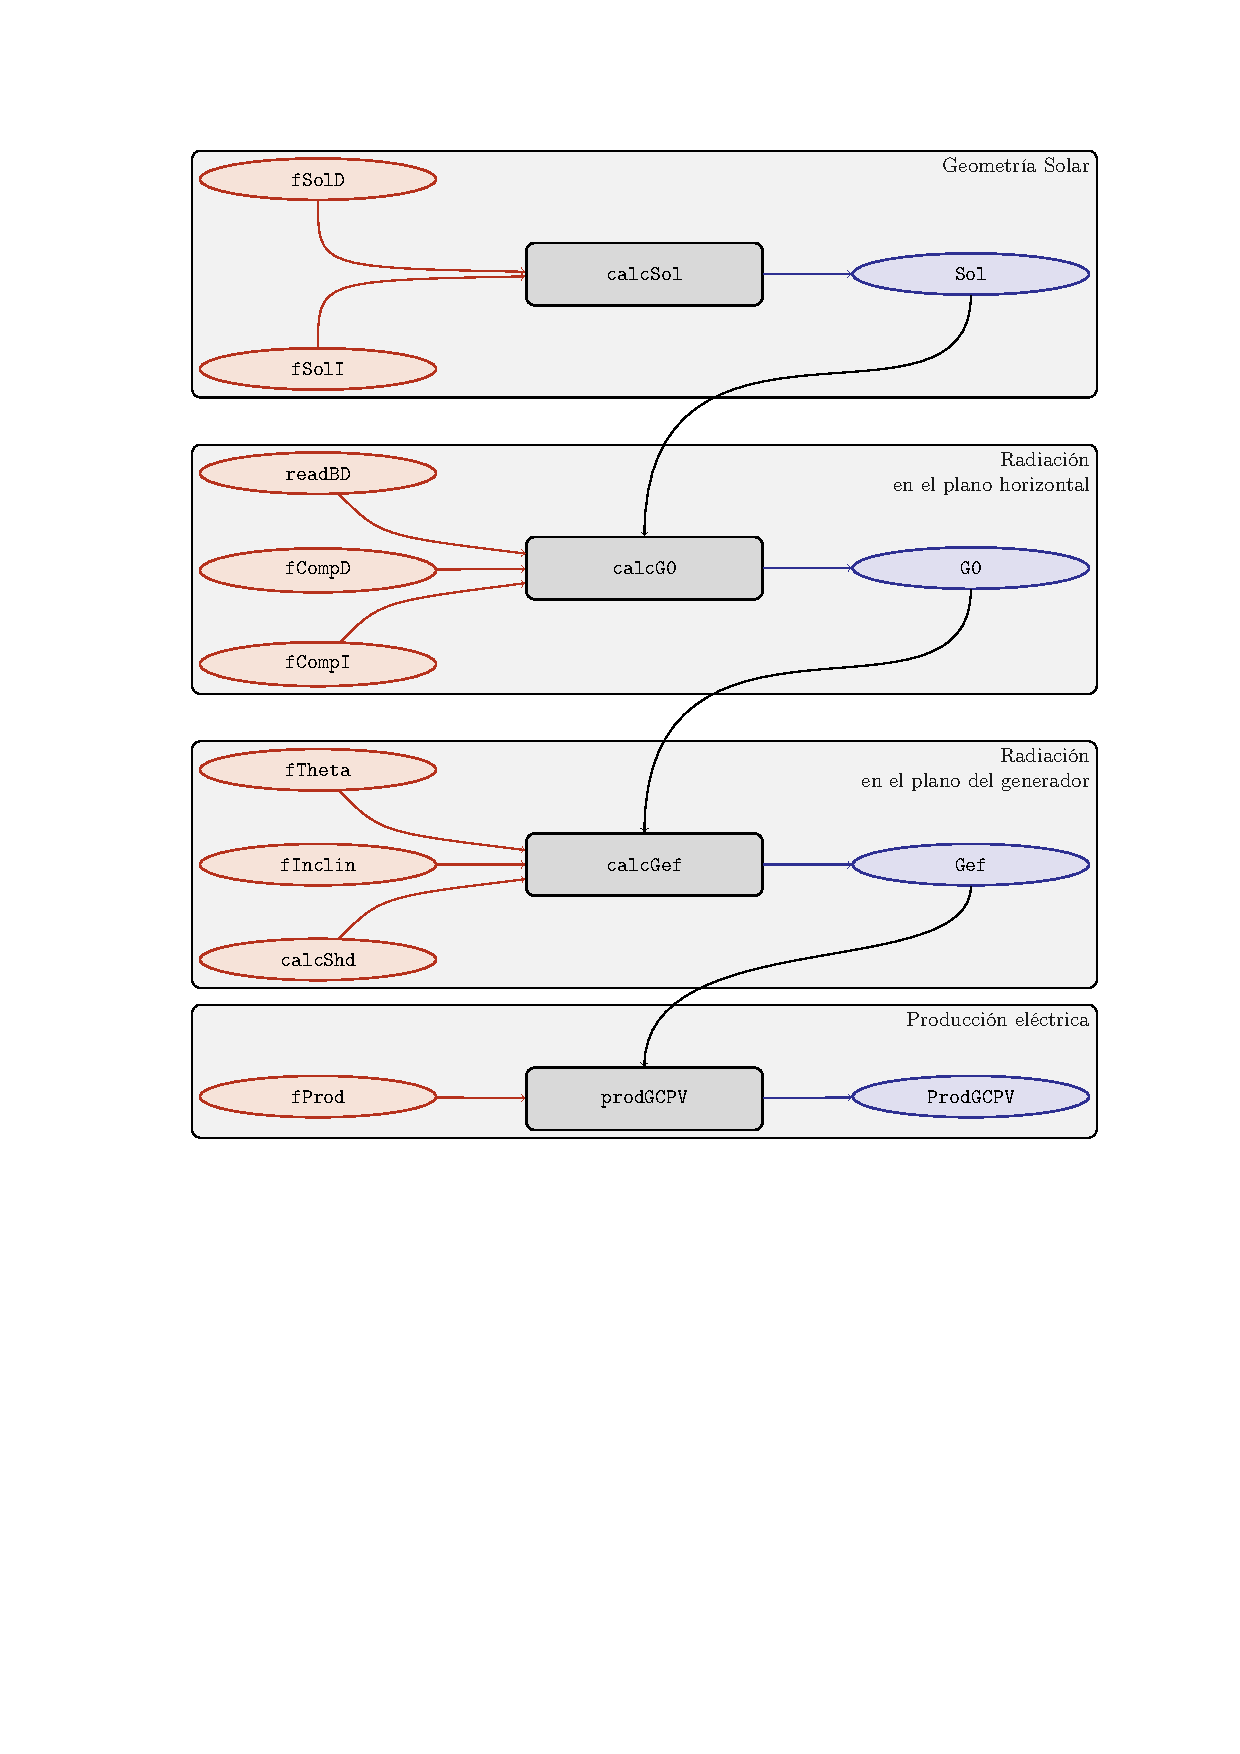
\includegraphics[scale=0.6]{figuras/procedure.pdf}
\caption{\label{fig:orgc6e945c}Proceso de cálculo de las funciones de \texttt{solaR2}}
\end{figure}
